% Put the caption to the left of the figure
% \begin{SCfigure}
%     \centering
%     \caption{Example of the semi-supervised few-shot learning setup. Training involves iterating through training episodes, consisting of a support set $\mathcal{S}$, an unlabeled set $\mathcal{R}$, and a query set $\mathcal{Q}$. The goal is to use the labeled items (shown with their numeric label) in $\mathcal{S}$ and the unlabeled items in $\mathcal{R}$ within each episode to generalize to good performance on the corresponding query set. The unlabeled items in $\mathcal{R}$ may either be pertinent to the classes we are considering (shown above with green plus signs) or they may be \emph{distractor} items which belong to a class that is not relevant to the current episode (shown with red minus signs). However note that the model doesn't actually have ground truth information as to whether each unlabeled example is a distractor or not, the plus/minus signs are shown only for illustrative purposes. At test time, we are given new episodes consisting of new classes not seen during training that we use to evaluate the meta-learning method.}
%     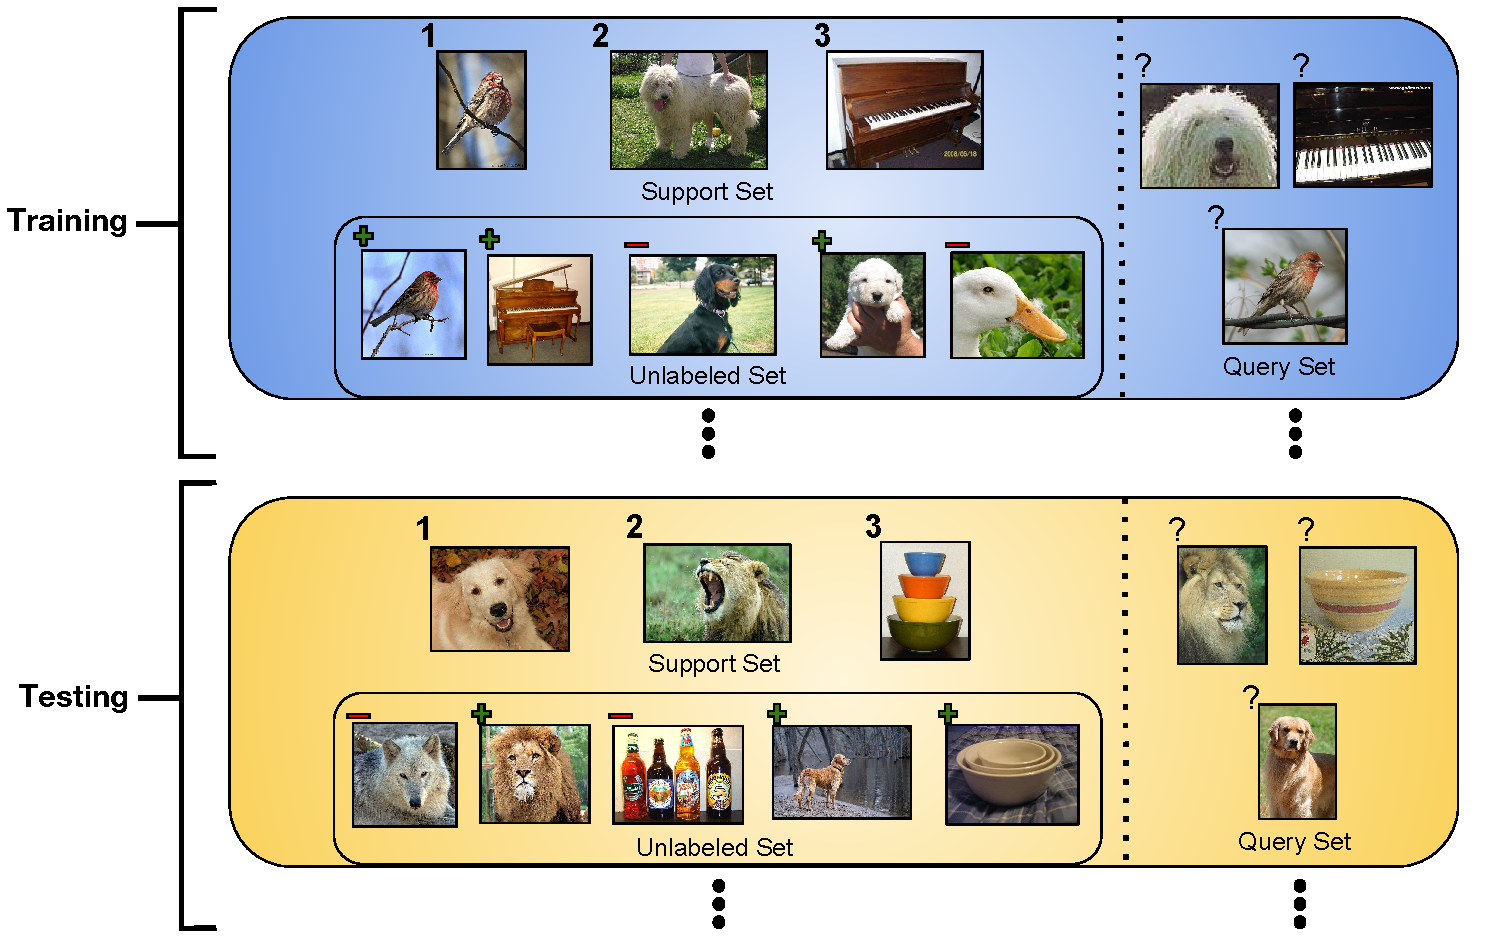
\includegraphics[width=0.77\textwidth]{figures/episode_setup.pdf}
%     \label{fig:episode_setup}
% \end{SCfigure}

\begin{figure}[ht]
    \centering
\iflatexml
    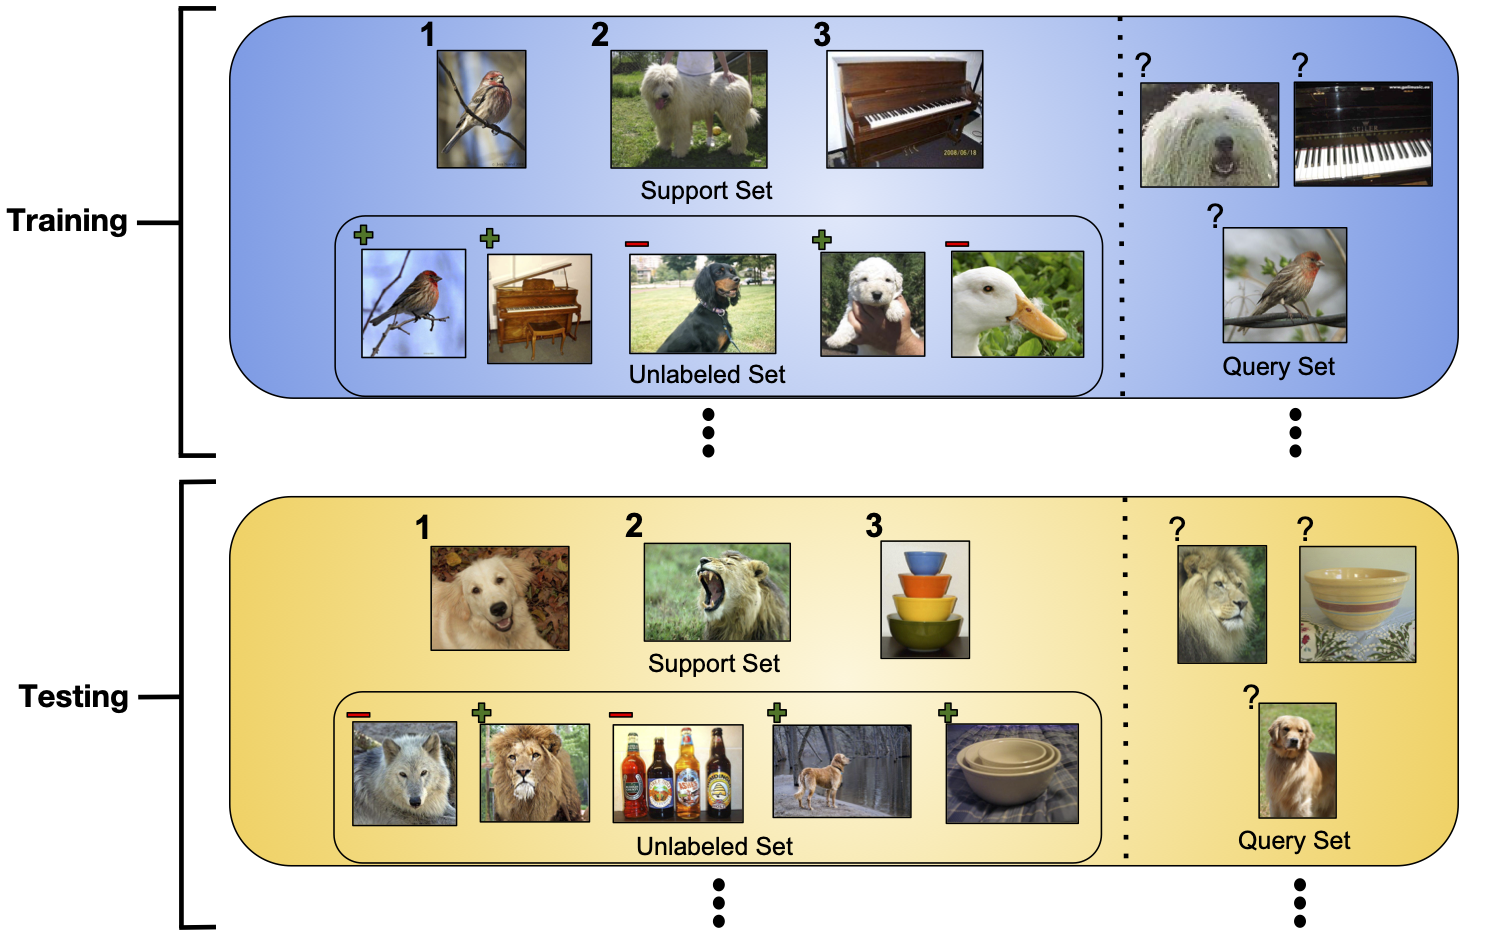
\includegraphics[width=6\textwidth]{figures/episode_setup.png}
\else
    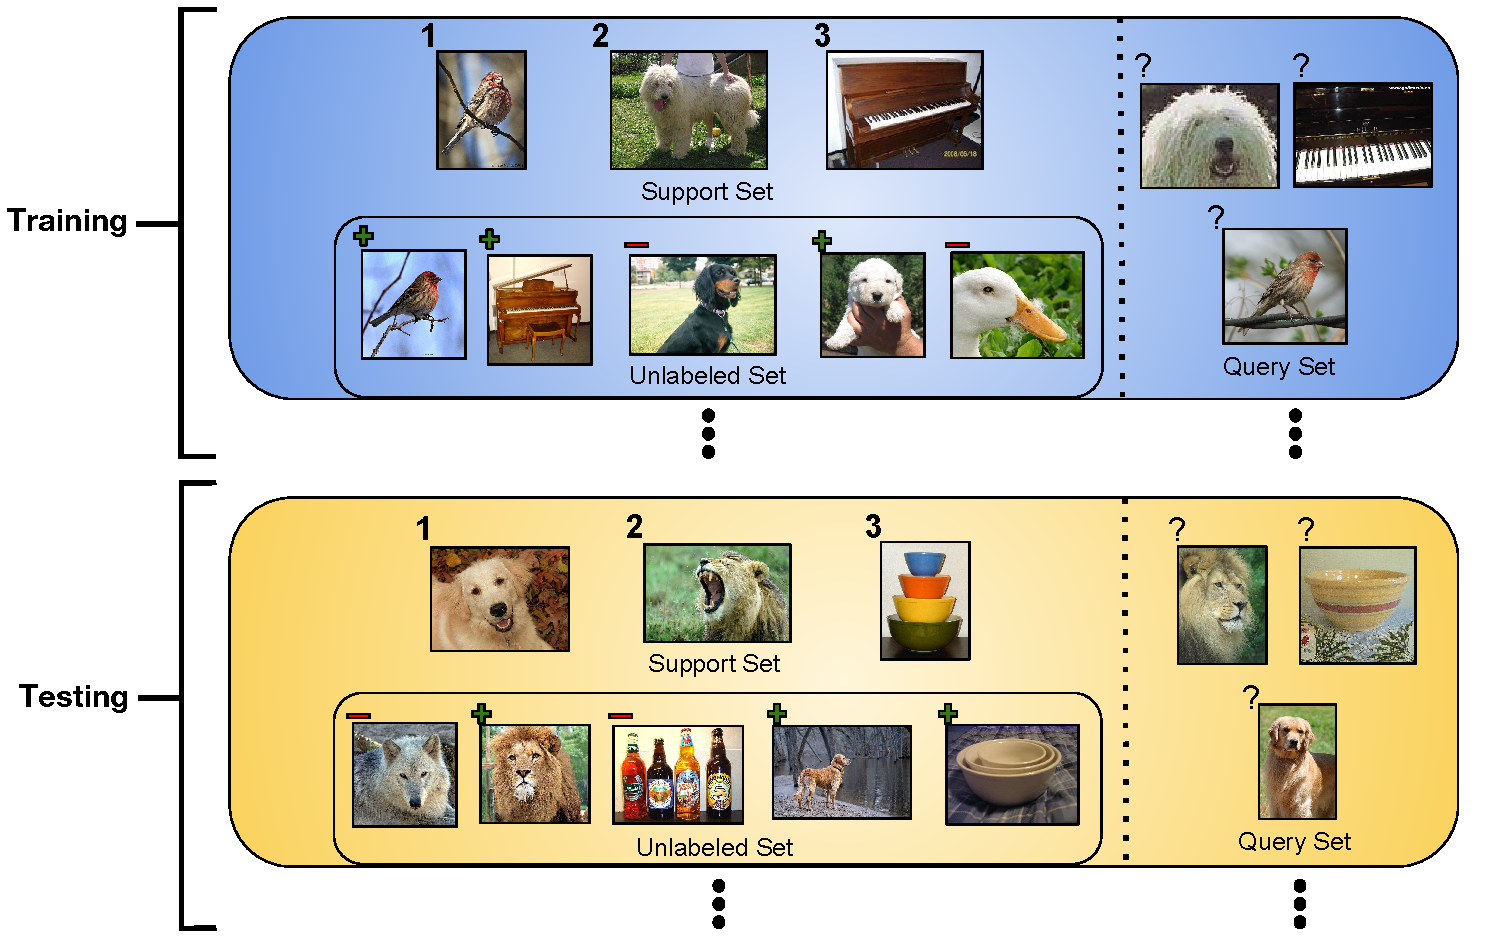
\includegraphics[width=0.77\textwidth]{figures/episode_setup.pdf}
\fi
    \caption{Example of the semi-supervised few-shot learning setup. Training involves iterating through training episodes, consisting of a support set $\mathcal{S}$, an unlabeled set $\mathcal{R}$, and a query set $\mathcal{Q}$. The goal is to use the labeled items (shown with their numeric class label) in $\mathcal{S}$ and the unlabeled items in $\mathcal{R}$ within each episode to generalize to good performance on the corresponding query set. The unlabeled items in $\mathcal{R}$ may either be pertinent to the classes we are considering (shown above with green plus signs) or they may be \emph{distractor} items which belong to a class that is not relevant to the current episode (shown with red minus signs). However note that the model does not actually have ground truth information as to whether each unlabeled example is a distractor or not; the plus/minus signs are shown only for illustrative purposes. At test time, we are given new episodes consisting of novel classes not seen during training that we use to evaluate the meta-learning method.}
    \label{fig:episode_setup}
\end{figure}